%%% Results %%%
\chapter{Evaluation \& Results} \label{ch:results}
This chapter presents the evaluation criteria for the endorsement model
proposed in chapter ~\ref{ch:method}. Based on which, the overall system design
and functionality will be evaluated and final results will be presented. 

\section{Evaluation Criteria}
To assess the fulfillment of requirements, a descriptive approach
based on the design evaluation method of \cite{hevner2010design} is used when
necessary. The system is not only reliant on the smart contract code and its
execution but also on the interaction theory discussed. For this, the
endorsement interaction will be simulated using an interaction graph simulation
tool neo4j~\footnote{\url{https://neo4j.com/}}. It will follow the study of graph topology and relevant subgraphs
to study the interactions and base the results on it. For this interaction, an
existing dataset from SNAP\cite{snapnets} is used. The details on the dataset
are presented in the respective section.  Given the time constraints, no form
of structural/unit testing was performed. The purpose of this project was a PoC
design to demonstrate reputation model as a use case via the use of smart
contracts and blockchain technology. Therefore, extensive experiment to
simulate a real-world usage was not performed. However, manual testing was done
during development using
ganache~\footnote{\url{https://github.com/trufflesuite/ganache}} and remix
environment~\footnote{\url{https://remix.ethereum.org/}}. Additionally, front-end for
endorsement interaction was also deployed to test simple function calls and
communicate from the web browser itself. 

\section{Fulfillment of User stories and Requirements}\label{fulfillment}
The method to examine fulfillment of user stories and requirement follows the
method used by \cite{Bergquist1107612} that uses Hevner's descriptive design
evaluation approach\cite{hevner2010design}. The table ~\ref{table:fulfillment}
presents the motivation for how the PoC fulfills the functional requirements. 
For the relevant smart contract code, refer to the appendix section. \\ 

The fulfillment of non-functional system requirements is discussed below:\\
\textbf{SmartContract Security:} Given the limited timeframe of this project
($\sim{4}$ months), not all security considerations were taken into account. As
part of fail-early
principle\footnote{https://blog.zeppelin.solutions/onward-with-ethereum-smart-contract-security-97a827e47702},
the contracts function code was ordered as conditions, actions, interactions
where relevant. A snippet of a function to demonstrate this is presented below. 

\begin{lstlisting}[language=Solidity]
	function joinNetwork(string _userName) public{
		//conditions: only allow unregistered participant
		require(!joined[msg.sender]);

		//actions
		joined[msg.sender] = true;
		
        //Interaction
		Participant memory newParticipant = Participant({
				identifier: msg.sender,
				name: _userName
        });
		participants.push(newParticipant);
        LogJoinNetwork(msg.sender, _userName);
        numberOfParticipants++;
        participantIndex[msg.sender] = numberOfParticipants-1;
    }
\end{lstlisting}

\begin{center} \label{table:fulfillment} 
	\begin{table}
		\begin{tabular} {| l | l | p{9cm} | }
		\hline
		\textbf{User}  & \textbf{Traceability}   & \textbf{Motivation for fulfillment} \\
		\hline
		\multirow{2}{*}{Endorser} & R1 & Any registered participant can make a
		call to endorse() function to send an endorsement to other registered
		participants on the network.      
		\\\cline{2-3} 
		& R2  & Any registered participant can call removeEndorsement()
		function just by providing the address of the endorsee they wish to
		remove.  \\\cline{2-3}
		& R3 & Each call to endorse() function updates the state variable of
		the current endorser and endorsee, storing and updating the respective
		state variables. i.e., nEG, nER, index. This function call also invokes
		updateEndorsee() function to update the endorsee information
		accordingly.  \\\cline{2-3}
		\hline
		\multirow{2}{*}{Endorsee} & R5.& The storage of personal information
		was not fully implemented by the endorsement PoC, therefore, editing
		personal information is irrelevant. However, change to pseudonym can be
		possible by just making a call to editProfile() by the participant.
		\\\cline{2-3}
		\hline
		\multirow{2}{*}{other users} & R4.1 & Anyone can make a call to
		computeImpact() function to get the final computed score of a
		participant based on public key hash registered on the endorsement
		network. \\\cline{2-3}
		& R4.2 &  Anyone can make a call to joinNetwork() function and become a
		registered participant of the network immediately.  \\\cline{2-3}
		\hline
	\end{tabular}
	\caption{Fulfillment of User stories and Requirements for Endorsement PoC}
\end{table}
\end{center}

\textbf{Reliability:}
The information of endorser, endorsee and their interaction is collected as
transaction data by the miners. A miner that is first to solve the hash value
of a block gets to write the list of transactions into a block and chain it to
the existing chain of blocks. The block-chain protocol ensures the immutability
of these list of transactions. i.e., Each block has a timestamp and a pointer
to the previous block. The public ledger ensures the verifiability of data
which can be checked by every node on the network.  Thus, the reputation score
stored on endorsement system can be said to be reliable. \\

%The reliability attribute refers to the tamper-proof,
%immutable traceability and verifiable nature of data. The blockchain
%infrastructure fulfills this requirement. The data in the context of
%Endorsement PoC is the endorsement interaction, list of endorsers and endorsees
%and the last computed endorsement impact of the respective user, etc. On a PoW
%setup, miners, the reliance is on miners to collect and put forward the list of
%transactions to the block. As long as a malicious attacker does not own more
%than 50\% of the processing power, PoW as a consensus mechanism is considered
%safe. The transactions once collected by miners and sent to the blockchain can
%be safely assumed to stay there as an immutable set of records. 
%

\textbf{Trust metrics correctly describe the actual trust of the nodes:} For
this requirement, an interaction graph is simulated, and different scenarios
are modeled that represents different possible behavior in the network.  Refer
to section ~\ref{sec:interaction} for this.

%%%%%%%%%%%%%%%%%%%%%%%%%%%%%%%%%%%%%%%%%%%%%%%%%%%%%%%%%%%%%%%
\section{Interaction graph} \label{sec:interaction}
For the simulation of user interaction in endorsement network and the resulting
impact value, a real-world data set was used. The dataset was extracted from
Bitcoin Alpha trust  \footnote{https://alphabtc.com/blockchain/} weighted
signed network which was mainly a who-trusts-whom network of people that trade
on Bitcoin Alpha platform. Participants on this network rated each other on a
scale of -10 to +10 where negative value represented total distrust whereas
positive value represented total trust. It consists of 3,783 nodes that made
24,186 edges out of which 93\% of the edges were marked as positive
edges\cite{kumar2016edge}.\\
\begin{figure}
	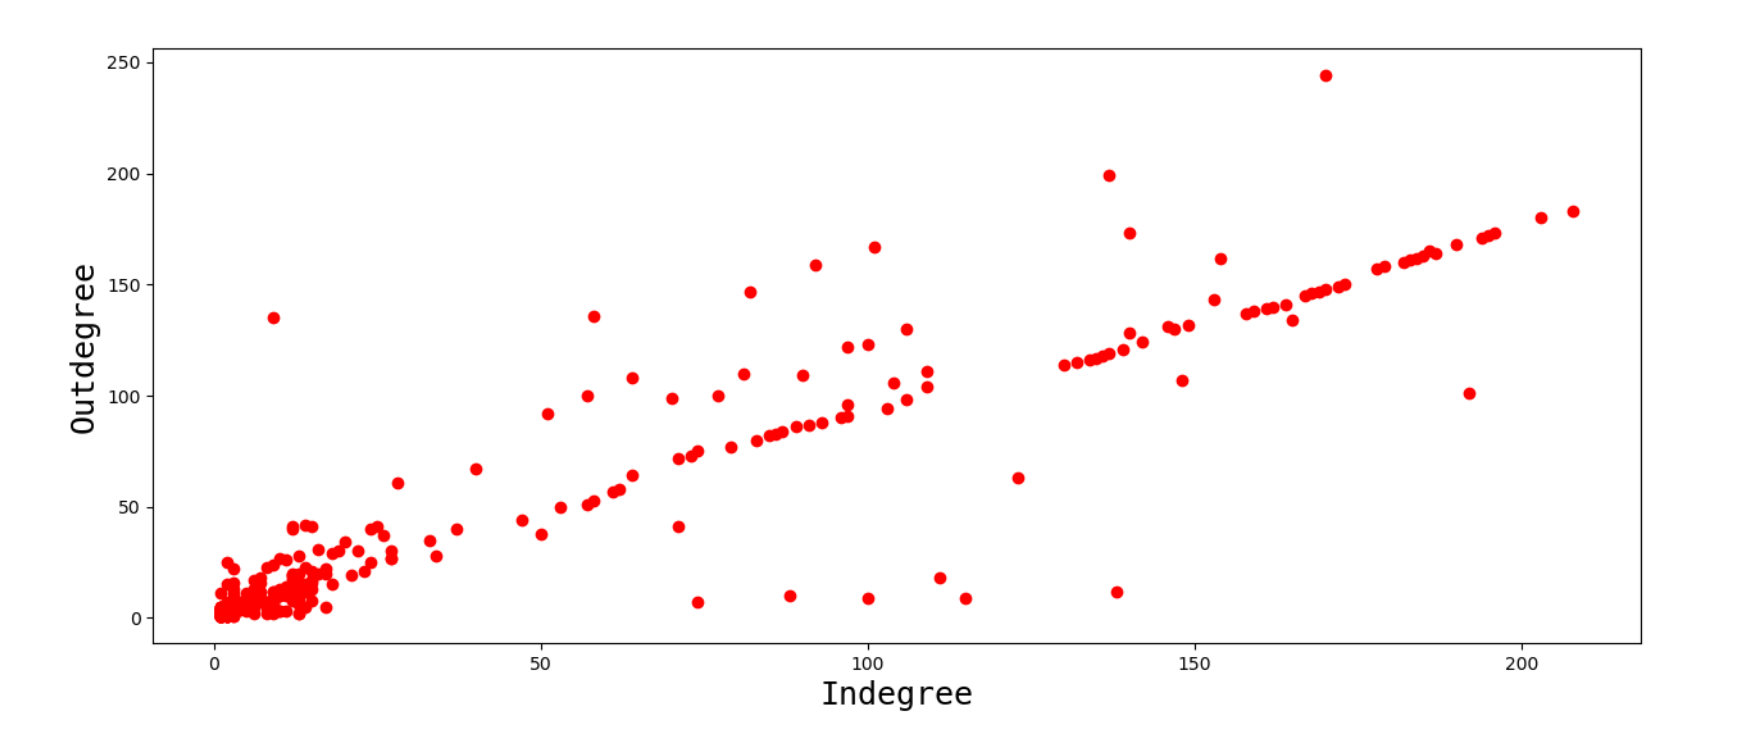
\includegraphics[width=0.95\textwidth]{Images/in_out.eps} 
	\caption{Given Vs. Received} 
	\label{inOut}
\end{figure}
The available information in the dataset for all the nodes was source, target,
rating, and timestamp. All of which is essential information for endorsement
network. The direction of endorsement is based on the source and target
information.  The timestamp information can help to decide on the order of
transaction occurrence in the network. This information is particularly
interesting for anomaly detection algorithm such as Net flow rate convergence
as discussed in \cite{buechler2015decentralized}.
Unlike the Bitcoin Alpha network that let users rate on a scale of -10 to +10
to demonstrate the strength of their trust towards other users. The endorsement
is more of a boolean decision problem. i.e., A user either endorses a specific
claim made by the entity or doesn't endorse. There is no range of values to
depict the strength or weakness. For making it a bit more relevant to
endorsement interaction, the existing dataset was filtered only to have edges
with a rating above +2. No negative edges were considered for the endorsement
simulation. As a result, the total number of nodes was reduced to 1677 with
4776 edges. Endorsement model was then applied to these nodes, and their total
endorsement impact was computed based on their edge weights. \\
The scores along with new findings are presented below: \\
\textbf{Total Endorsement Impact:} 
This value is based on the degree of connections and total received points for
each node. Surprisingly, there were 1175 nodes(70\%) whose final computed score
was equivalent to zero. On examining the nodes, it was found that all of these
nodes only had one incoming or outgoing connections. One requirement that was
required by the implementation was that a node needs to have a strictly greater
than one number of connections to be considered for impact score computation.
The distribution of indegree and outdegree can be seen in figure ~\ref{inOut}.
Having one connection is only considered a start in the network. The zero, in
this case, is not a representation of a non-trustworthy node, but a starting
node. Therefore, it can be assumed that 70\% of the nodes in the network are
new users. This computation leaves the network with only 502 nodes to account
for having a considerable impact value. 

\begin{tabularx}{\textwidth}{| X | X | X | X | X| X| }
  \hline
  \textbf{Node Label} & \textbf{nEG} & \textbf{nER} & \textbf{ratio} & \textbf{\acshort{TRP}} & \textbf{\acshort{TEI}} \\
  \hline 
  430  & 5  & 3  & 0.6 & 0 & 0 \\
  \hline
   761 & 2  & 2  & 1 & 0 & 0 \\
  \hline
  448  & 3  & 3  & 1 & 0 & 0 \\
  \hline
  676  & 2  & 2  & 1 & 0 & 0 \\
  \hline
  936  & 2  & 2  & 1 & 0 & 0 \\
  \hline
  \caption{Nodes with Impact zero because of the receivedpoints}
  \label{table:receivedpoints}
\end{tabularx}

\textbf{Total Received Points:}
The remaining 502 nodes had connections more than 1. Nevertheless, there were
still few nodes among them with impact value equivalent to zero. This is due to
another factor, received points, that the endorsement impact takes into
account. The relation between Total received points, and total endorsement
impact is shown in figure ~\ref{fig:receivedpointvsimpact}. This factor is more
or less similar to the prestige centrality metrics in a graph network. However,
in this case, the significance is not directly associated with the total
endorsement impact of the node it is connected to. Instead, the depleting
consumable point of a giving node accumulates to the received points to a
receiving node. The interaction subgraph is shown in figure
~\ref{fig:zeroimpact} for the discussed nodes behavior. The figure makes it
clear that even though the nodes 430, 761, 448, 676, 936 have a degree of
connection that is more than 1, their respective endorsers do not. Table
~\ref{table:receivedpoints} displays the state and scores of these nodes. 
%The behaviour of high impact node is shown in figure 
\begin{figure}
	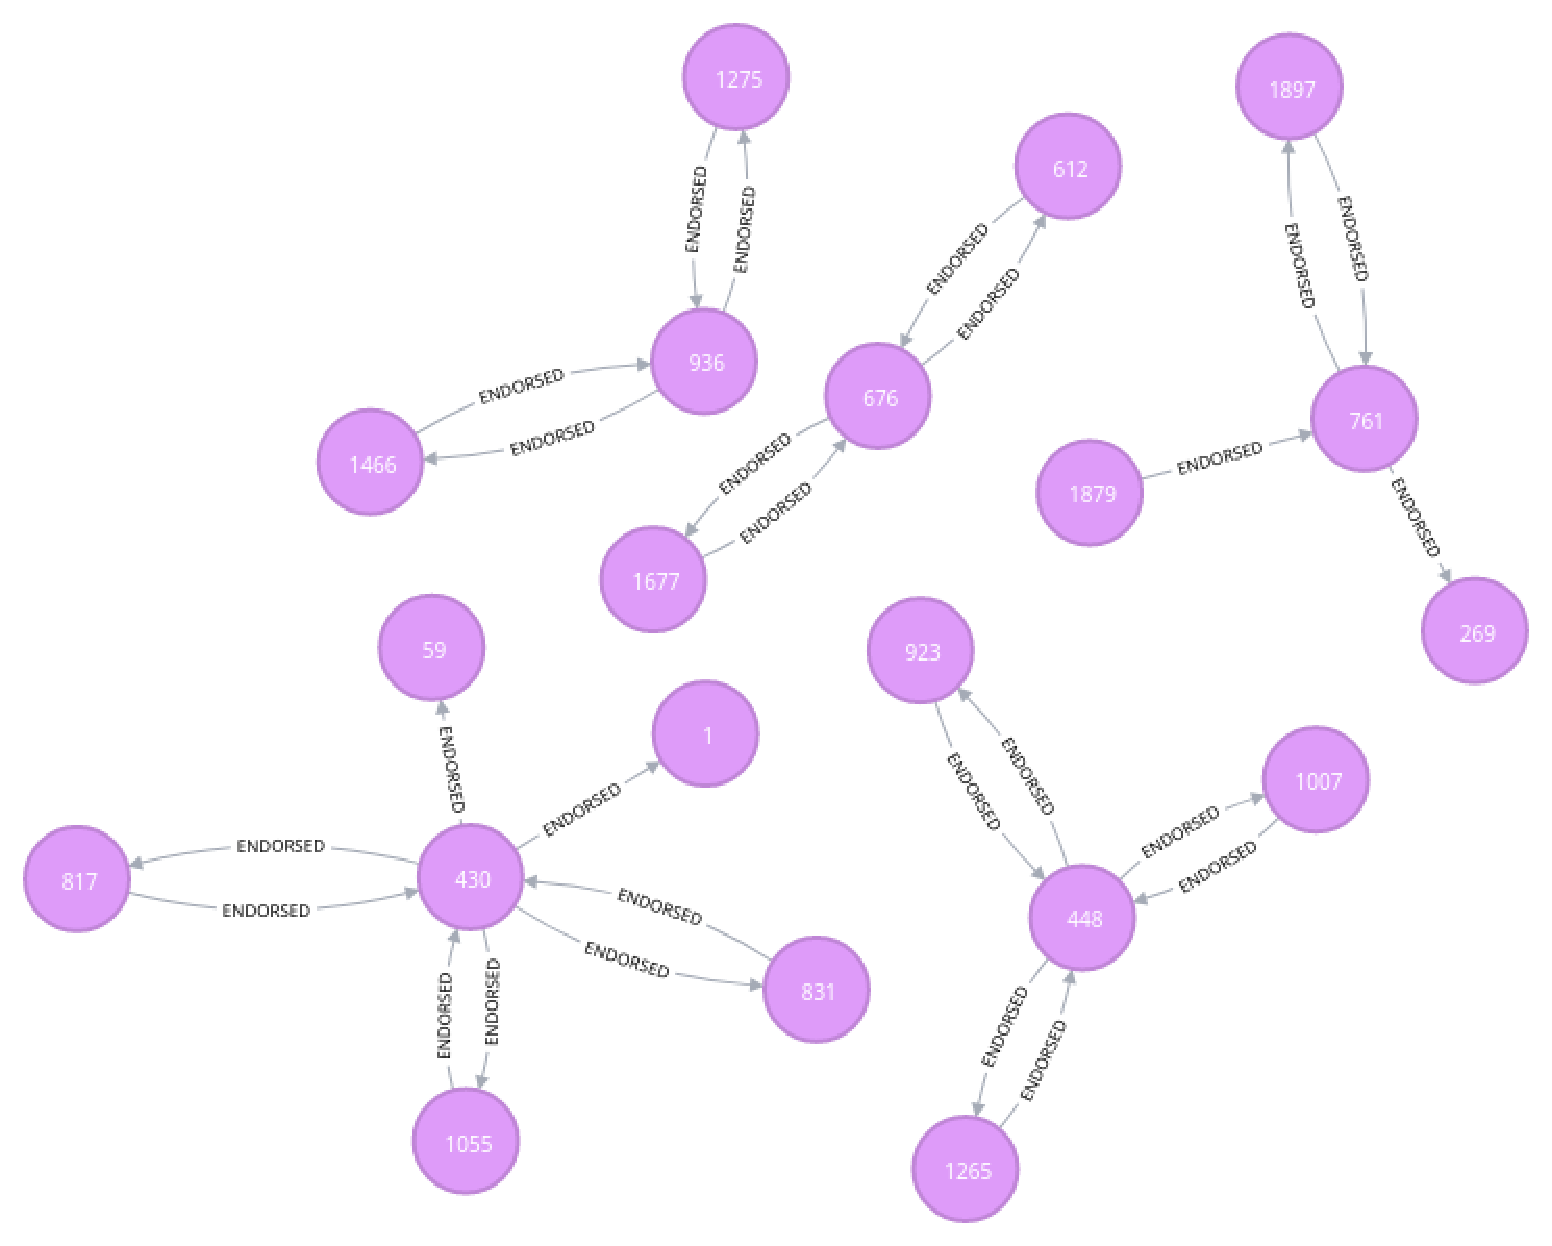
\includegraphics[width=0.95\textwidth]{Images/nodesWithImpactZero.eps}
	\caption{Interaction subgraph of nodes with impact zero}
	\label{fig:zeroimpact}
\end{figure}

\begin{figure}
	\includegraphics[width=1.0\textwidth]{Images/TRPVsTEIFontSize.eps}
	\caption{TRP vs. Total EDS Point}
	\label{fig:receivedpointsvsimpact}
\end{figure}
%\begin{figure}
%	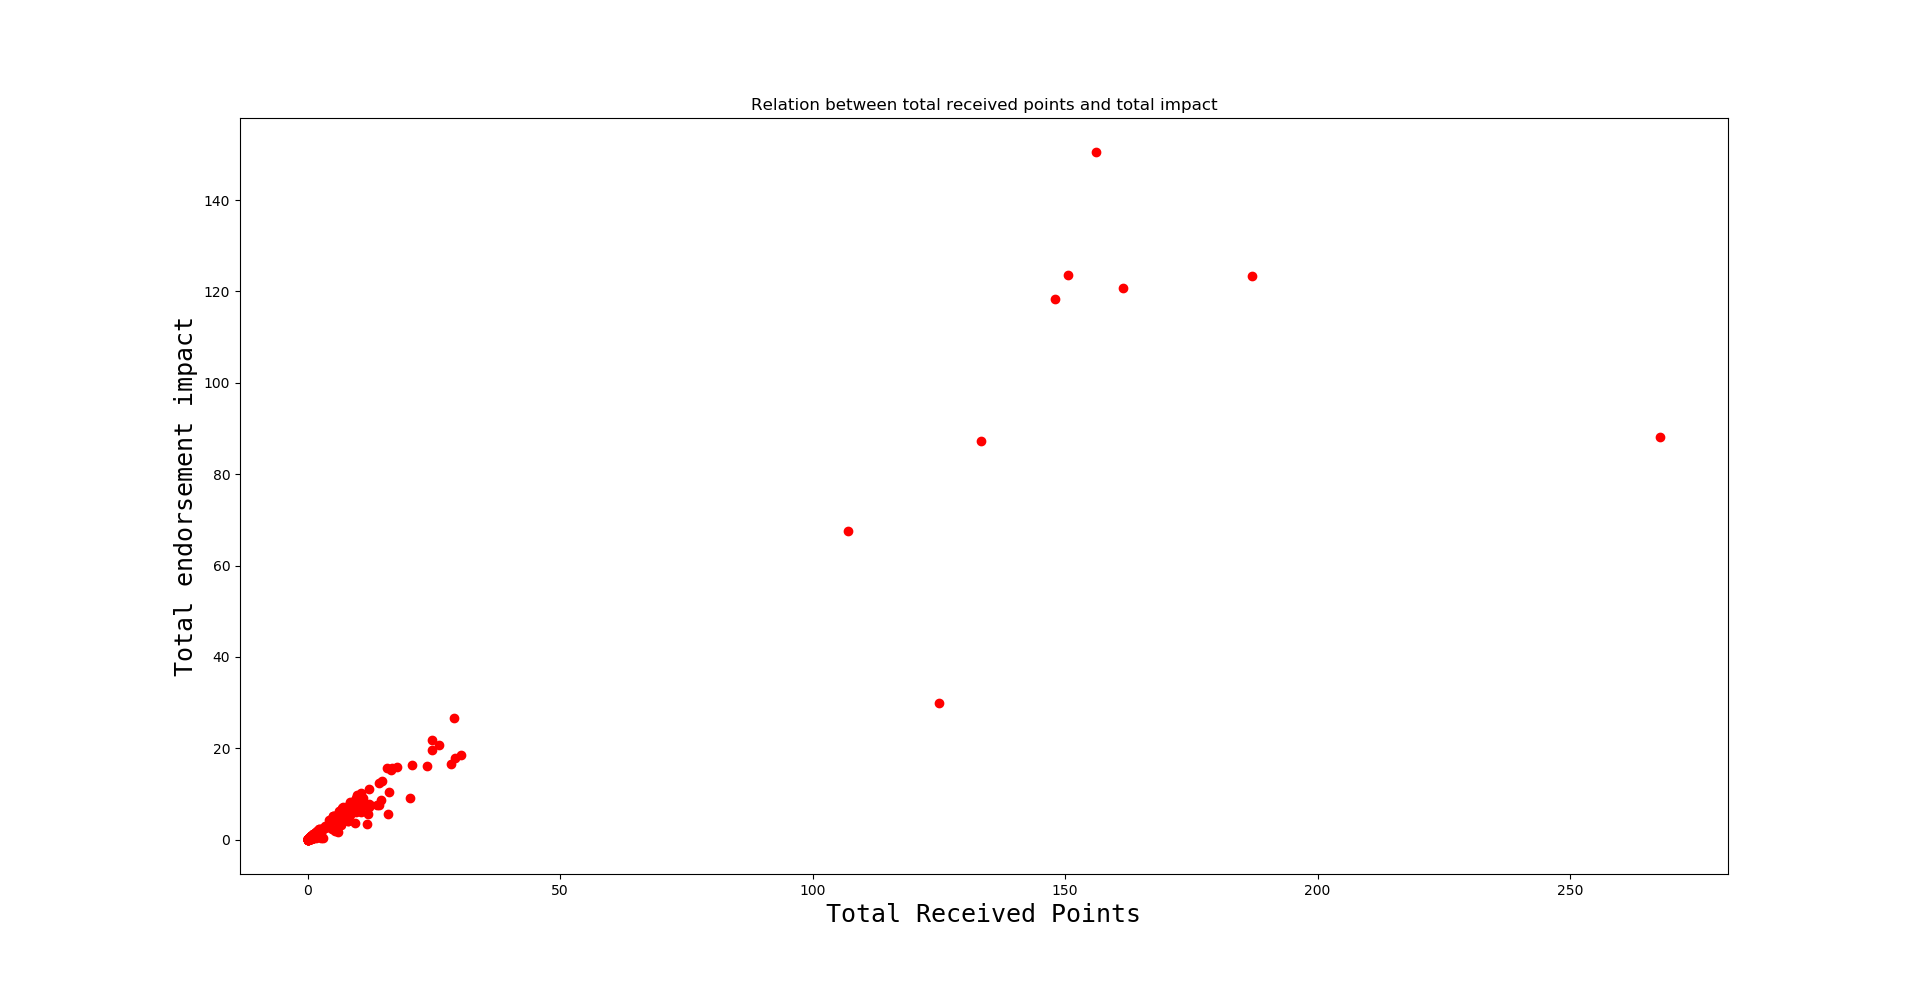
\includegraphics[width=1.0\textwidth]{Images/receivedPoints_impact_impactAboveZero.eps}
%	\caption{Received Points Vs. Total Endorsement Impact}
%	\label{fig:receivedpointvsimpact}
%\end{figure}

\begin{figure}
	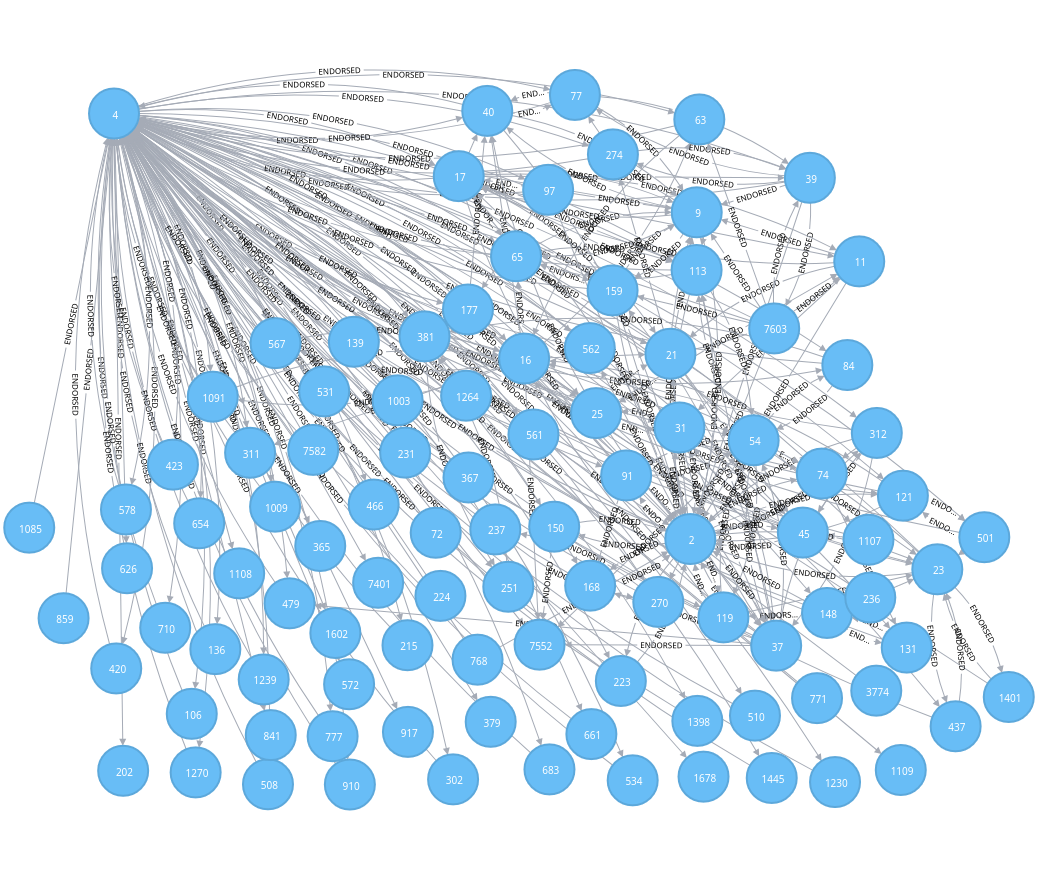
\includegraphics[width=1.0\textwidth]{Images/HighImpact_Node4.eps}
	\caption{High Impact Node}
	\label{fig:highImpactNode}
\end{figure}

\textbf{Ratio:}
Another significant factor that the Impact computation takes into account is
the ratio of indegree and outdegree. The table \ref{table:receivedpoints} makes
it clear that ratio alone is not enough to have a high impact. The figure
~\ref{fig:ratioimpact} shows the relation of ratio and total endorsement impact
over all nodes. One can infer that higher ratio does not imply a higher impact
but a higher impact most probably implies a higher ratio. As such, it is a
contributing factor in the long run. 

%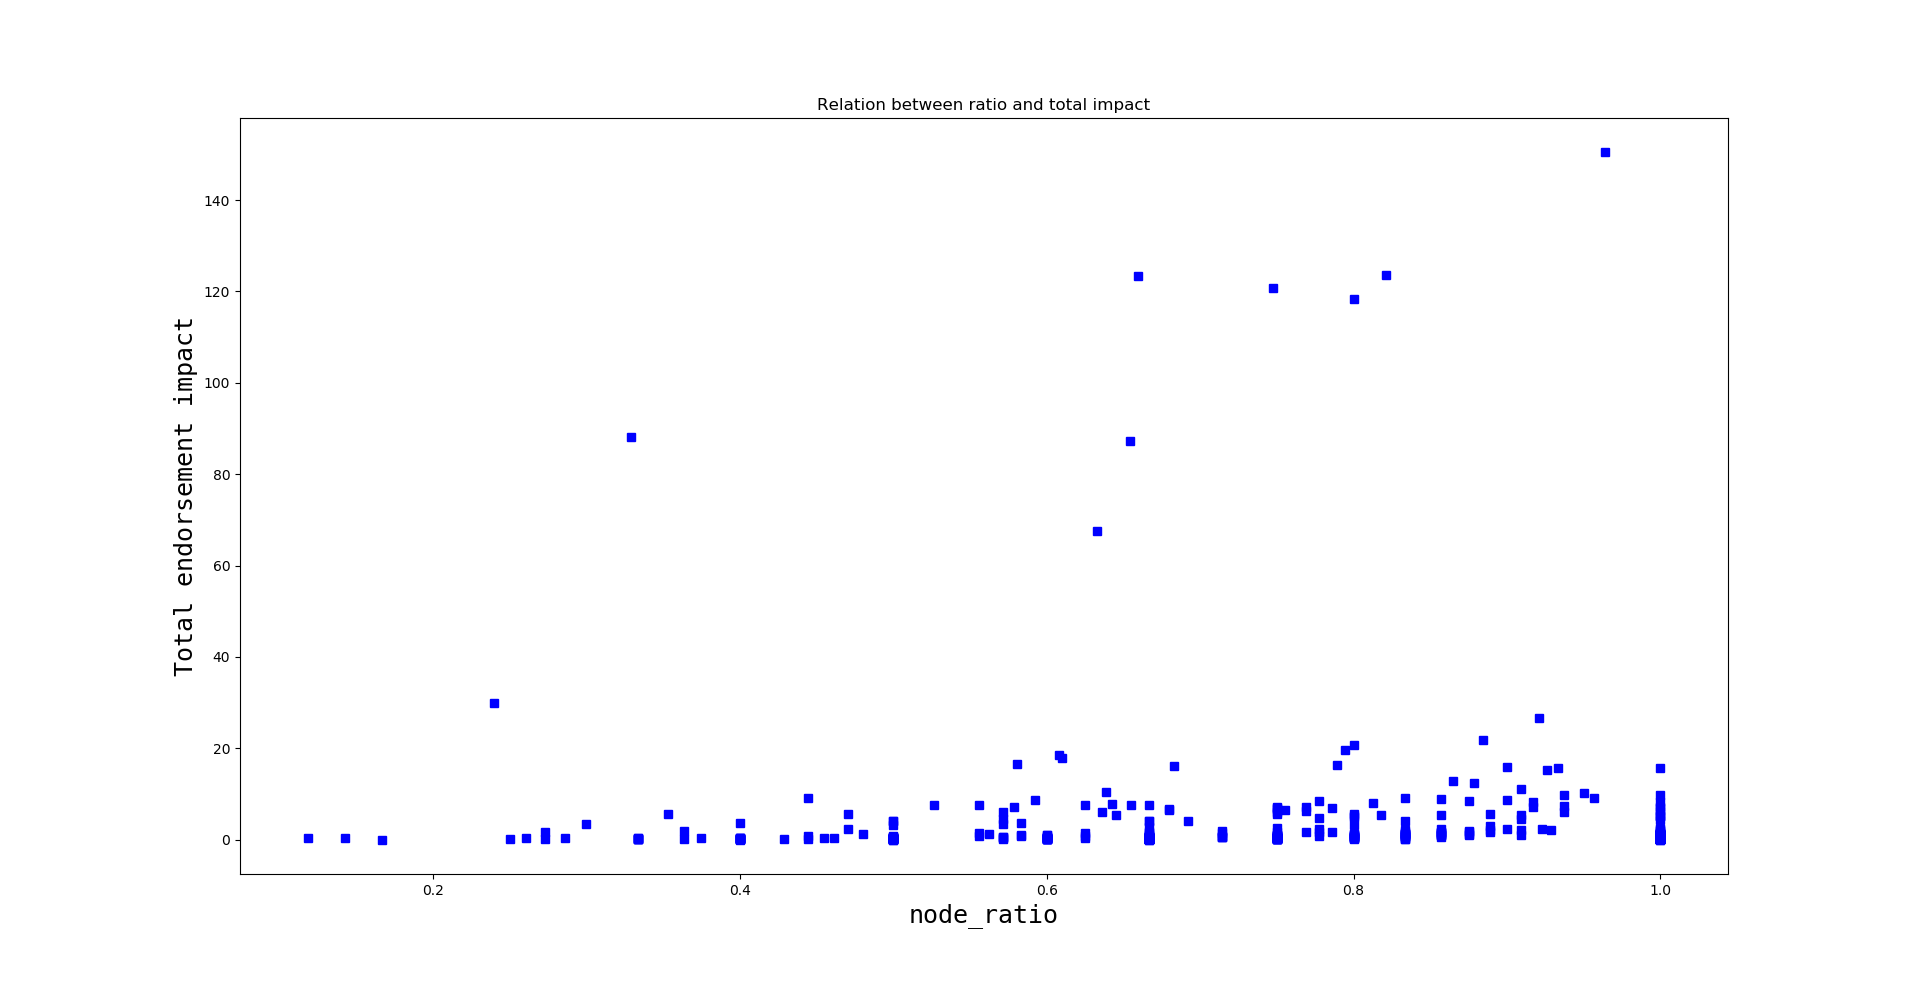
\includegraphics[width=0.95\textwidth]{Images/ratio_impact_impactAboveZero.eps}
\begin{figure}
	\includegraphics[width=0.95\textwidth]{Images/RatioVsTEIFontsize.eps}
	\caption{Relation of Ratio and Total endorsement impact}
	\label{fig:ratioimpact}
\end{figure}
Among the nodes that have maintained an above zero value for total endorsement
impact, the distribution of ranges is shown in table ~\ref{table:totalimpact}.
Majority of nodes have impact value within the range of 0-25. Only a few nodes
have managed to obtain a higher impact value.  For simplicity, one could
classify the impact value ranges as less trustworthy, average trustworthy and
more trustworthy. Based on the distribution table ~\ref{table:totalimpact},
0-55, 55-105 and 105-155 can be used for the mentioned classification. The term
maximum impact henceforth refers to the more trustworthy nodes, average impact
to average trustworthy and minimum impact refers to less trustworthy nodes. 
Figure ~\ref{fig:highImpactNode} gives the interaction subgraph of the most
impactful node for the provided network.
\begin{figure}
	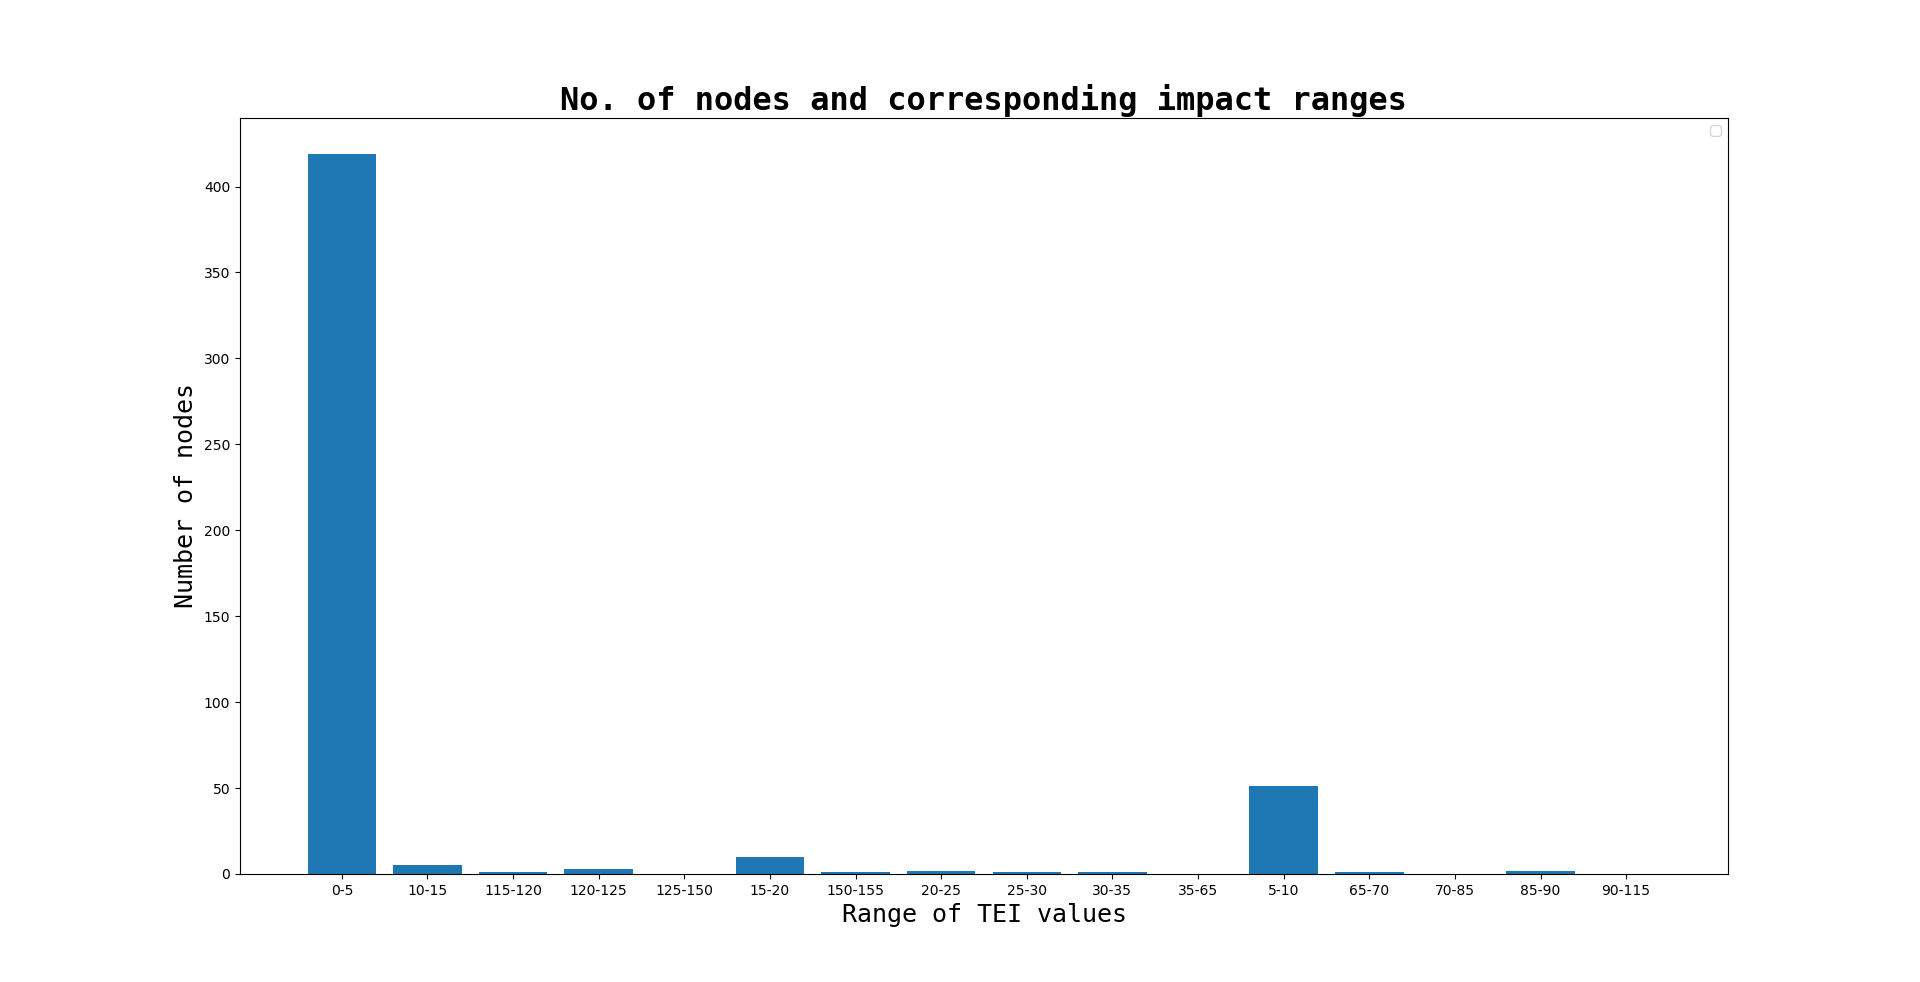
\includegraphics[width=1.0\textwidth]{Images/NoOfNodesVSImpactRanges.eps}
	\caption{table:totalimpact}
	\label{}
\end{figure}

%\begin{tabularx}{\textwidth}{| X | X | }
%  \hline
%   \textbf{No. of nodes} & \textbf{Impact Range} \\
%  \hline 
%  419  & 0-5  \\
%  \hline
%   51 & 5-10 \\
%  \hline
%  5 & 10-15 \\
%  \hline
%  10 & 15-20 \\
%  \hline
%  2 & 20-25 \\
%  \hline
%  1 & 25-30 \\
%  \hline
%  1 & 30-35 \\
%  \hline
%  0 & 35-65 \\
%  \hline
%  1 & 65-70 \\
%  \hline
%  0 & 70-85 \\
%  \hline
%  2 & 85-90 \\
%  \hline
%  0 & 90-115 \\
%  \hline
%  1 & 115-120 \\
%  \hline
%  3 & 120-125 \\
%  \hline
%  0 & 125-150 \\
%  \hline
%  1 & 150-155 \\
%  \hline
%  \caption{No. of nodes and the corresponding impact ranges}
%  \label{table:totalimpact}
%\end{tabularx}
\section{Total impact across several factors with different scenarios}\label{Allcases}
\begin{figure}[h]
	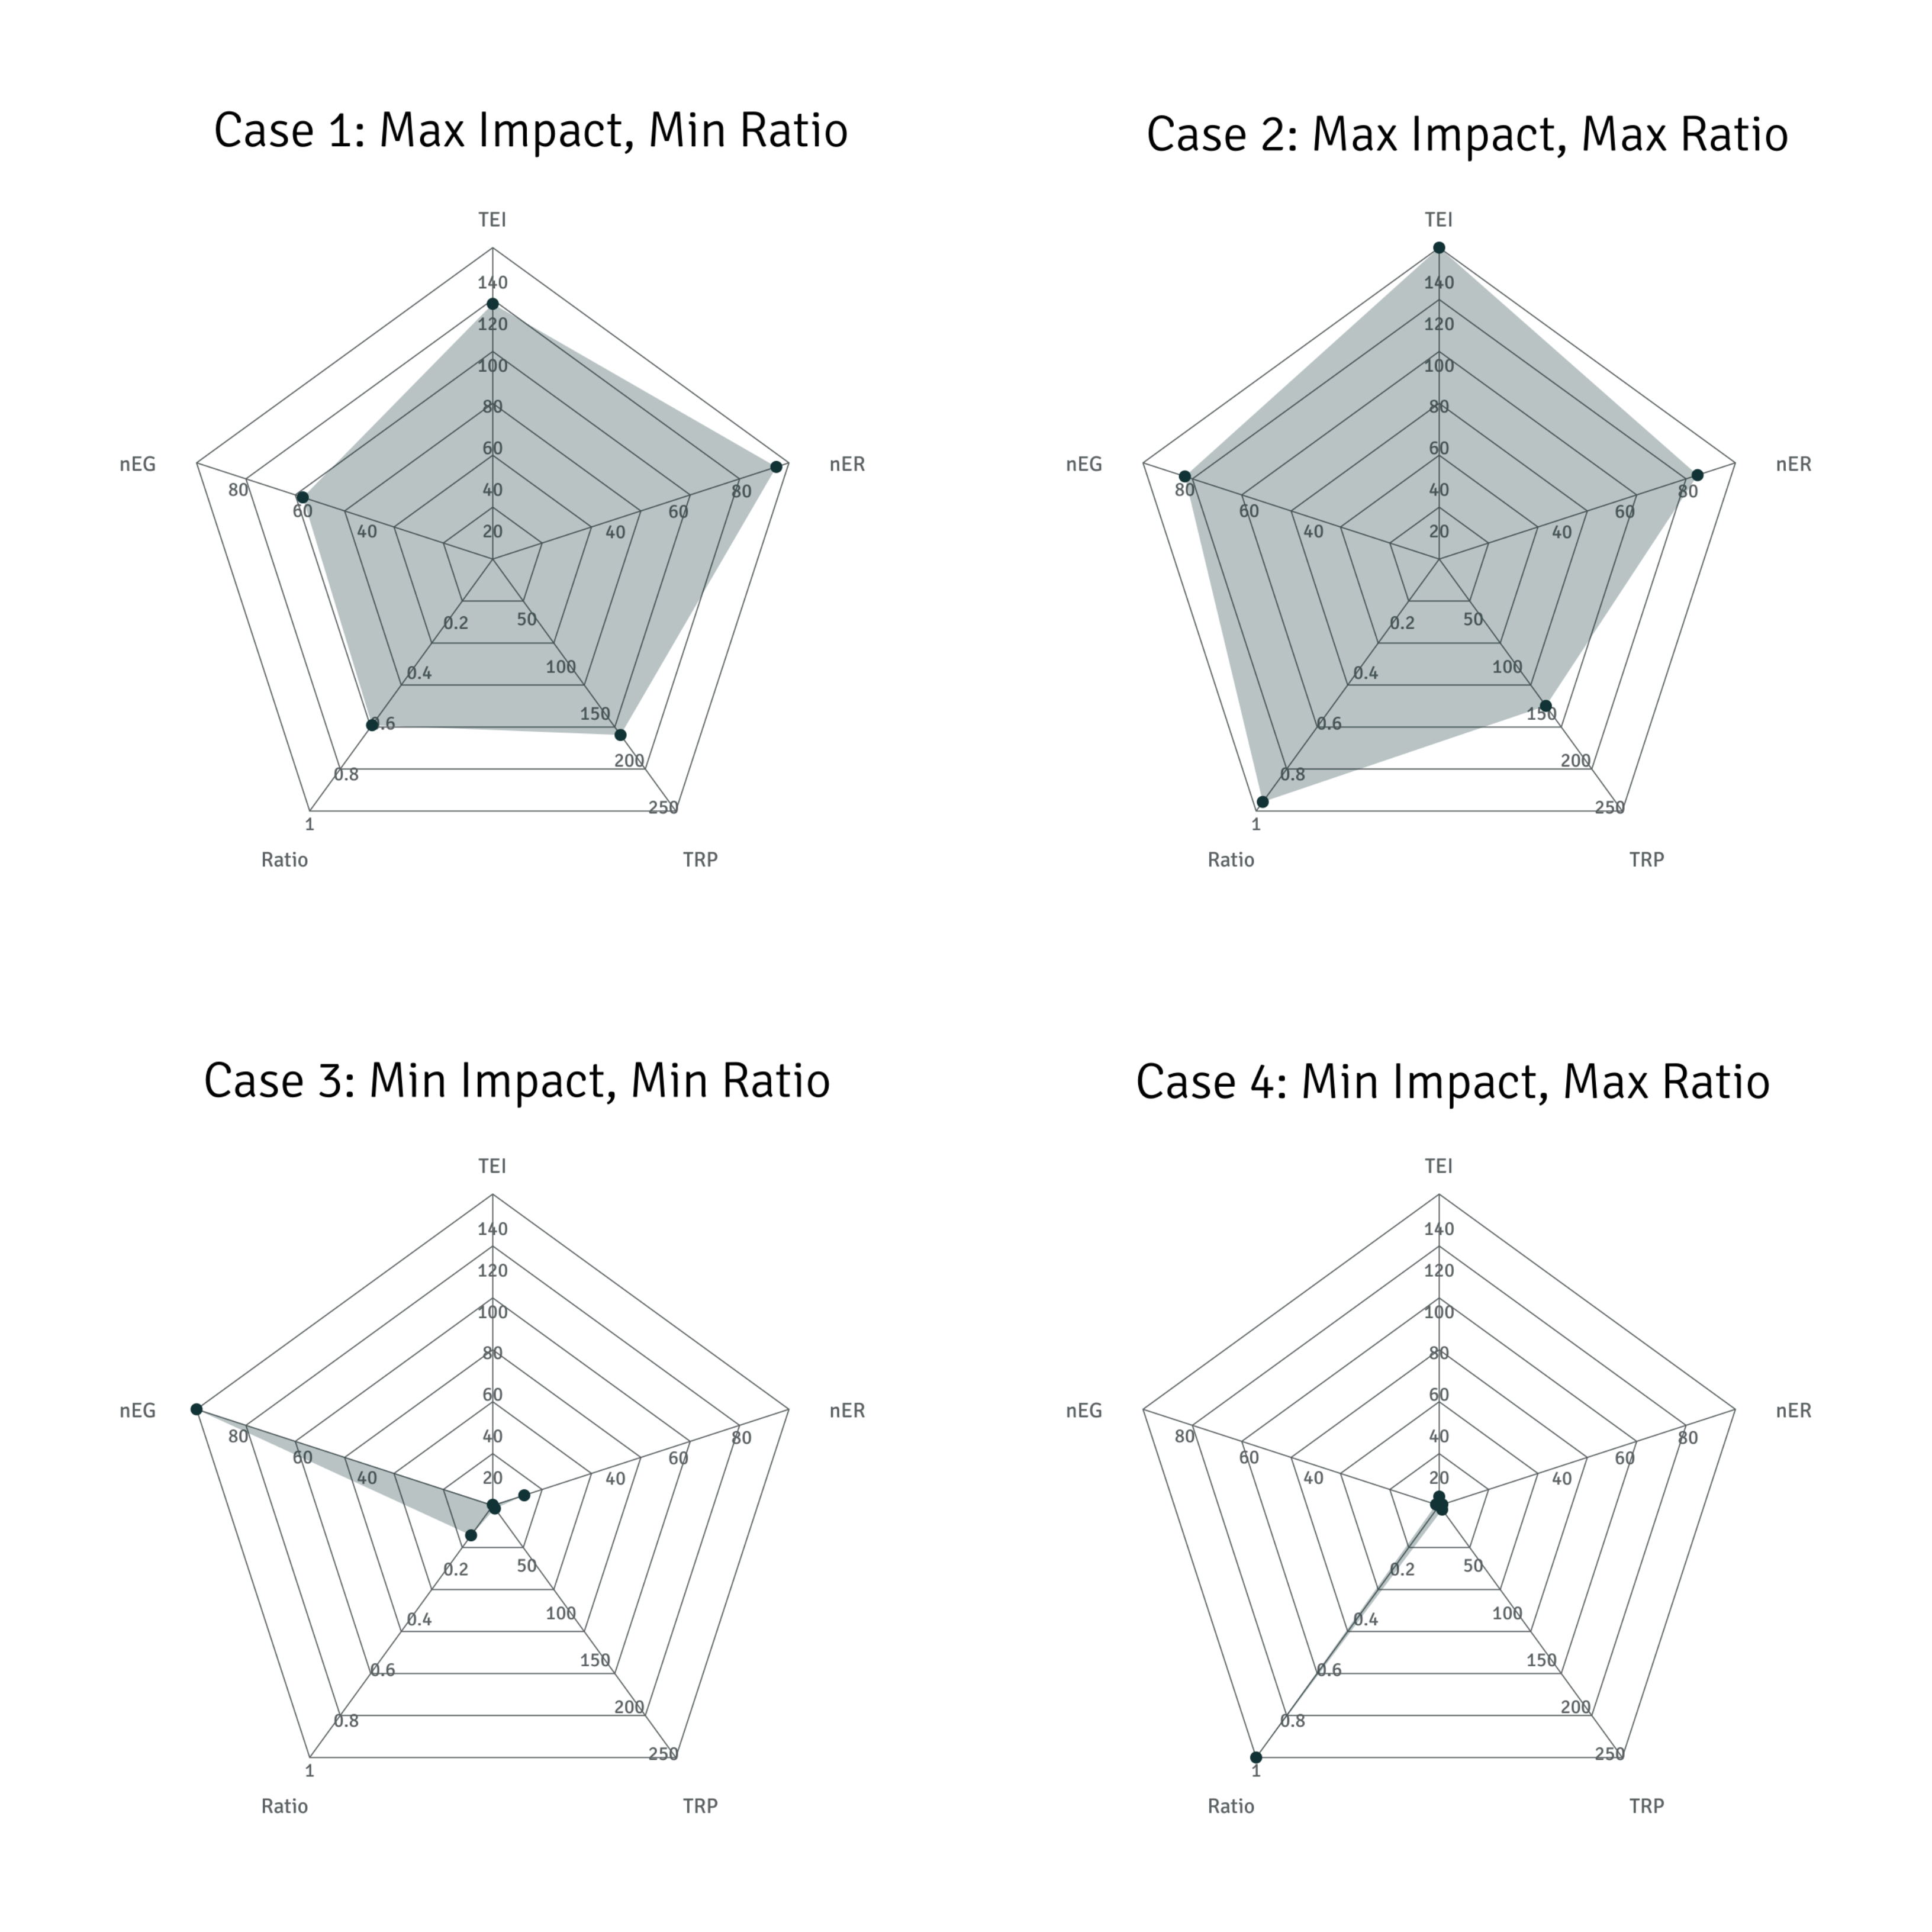
\includegraphics[width=0.8\textwidth]{Images/AllCases-acronyms.eps}
	\caption{Total Impact Across all factors}
	\label{fig:allCases}
\end{figure}
Different scenarios are considered to clarify further the relationship between
ratio and total endorsement impact. It seeks to answer the question such as why
a high ratio can both contribute to a high and low total endorsement impact and
vice-versa. Although only these two factors are mainly focused on creating
different cases, the study will show the effect of other factors and their
state as well. 
\subsection{Case1: Maximum Impact, Minimum Ratio}
All the nodes that got maximum impact value when computing the endorsement
impact are considered in this case. Among them, the nodes with the low ratio
are extracted to examine the behavior. As can be seen in figure
~\ref{fig:allCases}, the lowest ratio of a maximum impact node is 0.6. This
illustrates the behavior mentioned earlier that a maximum impact node most
certainly has a maintained ratio. 
\subsection{Case2: Maximum Impact, Maximum Ratio}
A maximum ratio of a node with a maximum impact should be the maximum ratio
possible in the network. This behavior is the best case scenario where a node
is actively participating both as an endorser and an endorsee. The data is
taken using the same approach as in case1 for this scenario as well. The
behavior of such a node is depicted in figure ~\ref{fig:allCases} Case2. The
value across all dimension is equally distributed. 
\subsection{Case3: Minimum Impact, Minimum Ratio}
A minimum impact node is the one that is not an active participator in the
network across all dimension as required. For this category, all the nodes from
minimum impact region were taken. From those nodes, the node with the minimum
impact is taken to show the behaviour as shown in figure ~\ref{fig:allCases}
Case3. It can be seen that the node has only actively involved in giving out
endorsements but received relatively low connections. As such, neither the
ratio or the impact is significant for this node. This behavior is typical of
an extreme one-way connection. 
\subsection{case4: Minimum Impact, Maximum Ratio}
Table ~\ref{table:receivedpoints}  and figure ~\ref{fig:ratioimpact} has
already demonstrated this form of behavior as well. From the minimum impact
nodes, the node with the maximum ratio is taken to simulate an interaction that
looks like figure ~\ref{fig:allCases} case 4.

\section{Threat Model}\label{sec:threatModel}
An honest peer in the endorsement system has scores distributed across all
factors as shown by figure ~\ref{fig:allCases} in case2. Similarly, a malicious
peer is the one that has high score across one dimension which is shown by case
3.\\
The relevant threat scenarios for the proposed system can be described as
following: \\
\textbf{Individual and collective malicious peers\cite{marmol2009security}:}
A malicious peer is always supposed to provide inferior services in the
transactional network. Similarly, a malicious collective is formed by a group
of malicious peers that give a good rating to each other with the intent of
inflating their trust score. This can be detected by other peers based on
feedback/rating. Once detected, the peer will have an endorsement impact
reduced by 50\% and the endorsers of the node will have the total impact
reduced by 25\%.

\textbf{Sybil Attack:}
The endorsement network addresses Sybil attack by requiring the endorsers of a
peer to have high TEI as well. A peer can create multiple Sybil identities and
self-interact to send a large number of endorsements directed to themselves.
However, being endorsed by the set of endorsers with a zero or low impact does
not contribute towards a better global score for that node as discussed
earlier. Thus, a peer that creates multiple identities is required to maintain
the score across all factors for all pseudonymous nodes thereby increasing the
cost of maintaining global value for all nodes.

%A peer can create multiple Sybil identities and interact with self to send a
%large number of endorsements directed to themselves. The cost of creating a new
%identity and joining the network is not as high.  The gas cost as mentioned in
%section ~\ref{subsec:design_considerations} plays a significant role in limiting this
%behavior. However, it is a naive assumption and merely relying on it may not be
%the best approach.  Therefore, an algorithm such as max-flow, min-cut can be
%used to analyze the network and distinguish the edge that forms the edge
%between honest and Sybil cluster. Similarly, Net flow rate convergence
%algorithm as proposed by \cite{buechler2015decentralized} can also be used to
%detect anomaly by computing the net flow of the subgraph. Once detected, the
%peers are penalized as mentioned above.

\textbf{Whitewashing:}
Whitewashing~\cite{feldman2006free} is when a peer with a bad reputation score
on a P2P network tries to exit the system and starts afresh as an entirely new
user. In case of endorsement system, a new user can never have an impact score
higher than an old user. Assuming that a malicious peer was detected and
penalized, the penalty is a certain percentage of the obtained score. As such,
an old user will always an impact value greater than zero. The new user, on the
other hand, will start with a full consumable point but a zero impact value. To
be considered for impact computation step, the peer needs to make strictly
larger than one connection.  Since the value is decreased in percentage. A new
user will only receive a consumable point but has a zero impact when entering
the network. The design requires that a peer make strictly more than one
connection to be considered for impact computation step. Thus, white-washing is
a discouraging attack in the endorsement model. 


\textbf{Freeriders:}
In a P2P network that provides service, free-riders indicates the peers that
only take services but do not participate equally in uploading files. In
endorsement system, they can denote the peers that have high outdegree and
negligibly low incoming connections. As shown by ~\ref{sec:interaction}, doing
so doesn't contribute to a high total impact value.

%\section{Blockchain: Gas Consumption, Block size, Transactions}
%Ethereum  specific concepts:
%As mentioned earlier, executing any operation on Ethereum costs some amount of
%gas. The total amount of transactions that can be included in an Ethereum block
%is therefore not determined by the size but by the amount of gas consumed by
%them. The block limitation is about 4 million gas per block.  The current block
%according to etherscan\footnote{http://etherscan.io/} is Block number 5778648
%with a total of 155 transactions recorded in it. The time between the previous
%block and the current block is around 11 seconds. Thus, the network throughput
%based on this data is around 11 transaction per second. The average block time is 17 seconds which is dynamically adjusted based on how fast or slow 
%





%The gas consumption for the transactions in endorsement contract is based on
%the tests performed on Rinkeby test network and remix environment. The gas
%price and gas limit are based on the statistics from the main ethereum network
%\footnote{https://ethgasstation.info/index.php}. The gas cost to join the
%endorsement network is 142927 units of gas and to send an endorsement is 203746
%units of gas. Recommended safe low value for the gas price is 2
%Gwei(0.000000002 eth). 
%The block size limitation in ethereum is about 4 million gas per block.
%Therefore, the total amount of transactions is not determined by its size but
%by the amount of gas it consumes. The current block according to
%etherscan\footnote{http://etherscan.io/} is Block number 5778648 with a total
%of 155 transactions recorded in it. The time between the previous block and the
%current block is around 11 seconds. Thus, the network throughput based on this
%data is around 11 transaction per second. 










%\section{Analysis}
%\section{Measurement}
%\section{Comparison}

% Presentation of results and case-study data 
% An application of the methodology is unfolded and results are presented using for example via Charts, Diagrams, Figures and Tables 
% The work is conducted in accordance with the method described earlier. Results are presented in an analytical way.
